% begin module vertical-asymptote-ex10
\begin{frame}
\begin{example}[Example 10, p. 74]
Find the vertical asymptotes of $f(x) = \tan x$.
\begin{columns}[c]
\column{.45\textwidth}
\uncover<10->{%
\ \ 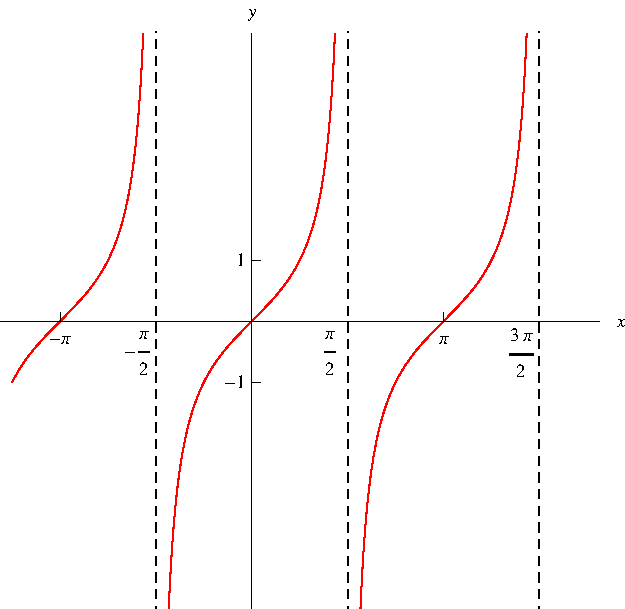
\includegraphics[height=5cm]{limits/pictures/app-d-tan.pdf}%
}%

\uncover<10->{%
\begin{center}
$y = \tan x$
\end{center}
}%
\column{.55\textwidth}
\begin{itemize}
\item<2->  $\tan x = \sin x/\cos x$.  
\item<3->  Potential vertical asymptotes where $\cos x = 0$.  
\item<4->  $\cos x \rightarrow 0^+$ as $x\rightarrow (\pi /2)^-$ and $\cos x\rightarrow 0^-$ as $x\rightarrow (\pi /2)^+$.
\item<5->  $\sin x$ is positive around $\pi /2$. 
\item<6->  $\lim_{x\rightarrow (\pi /2)^-} \tan x = \infty$.
\item<7->  $\lim_{x\rightarrow (\pi /2)^+} \tan x = -\infty$.
\item<8->  So $x = \pi/2$ is a vertical asymptote.
\item<9->  Similar reasoning works for $x = \pi/2 + n\pi$, where $n$ is any integer. 
\end{itemize}
\end{columns}
\end{example}
\end{frame}
% end module vertical-asymptote-ex10
